\documentclass[letterpaper, 10pt]{article}
\usepackage{amsmath, bbm}
\usepackage{amssymb, amsthm}
%\usepackage{mathptmx}
%\usepackage[LY1]{fontenc}
\usepackage{fancyhdr}
\usepackage{graphicx}
\usepackage{subfigure}
\usepackage{verbatim}
\usepackage{array}
\usepackage{hyperref}
\usepackage[squaren]{SIunits}
\usepackage{color}

\topmargin 0in
\headheight 0.0pt

\headsep 0. in
%\bottommargin 1in
\oddsidemargin 0.0 in
\evensidemargin 0.0 in
\textwidth 6.5 in
\textheight 9 in

\renewcommand{\headrulewidth}{0pt}
\newcommand{\tmop}[1]{\operatorname{#1}}
\newtheorem{lemma}{Lemma}
\newtheorem{theorem}{Theorem}
\newtheorem{definition}{Definition}
\newtheorem{claim}{Claim}
\newtheorem{proposition}{Proposition}


\newcommand{\neal}[1]{\textcolor{red}{Neal: #1}}
\newtheorem{corollary}{Corollary}
\newtheorem{fact}{Fact}
%%%%%%%%%%%%%%%%%%%%%%%%%%%%%%%%%%%%%%
%%       EDIT THESE VARAIBLES       %%
%%%%%%%%%%%%%%%%%%%%%%%%%%%%%%%%%%%%%%


%%%%%%%%%%%%%%%%%%%%%%%%%%%%%%%%%%%%%
%%%%%%%%%%%%%%%%%%%%%%%%%%%%%%%%%%%%%%
    \newcommand\independent{\protect\mathpalette{\protect\independenT}{\perp}}
    \def\independenT#1#2{\mathrel{\setbox0\hbox{$#1#2$}%
    \copy0\kern-\wd0\mkern4mu\box0}} 
    \numberwithin{equation}{section} 
\author{Neal Wadhwa}
\title{Phase Model for Motion Dynamic Range Compression}
\date{January 28, 2014}
\begin{document}
\newcommand{\D}{\mathcal{D}}
\newcommand{\pr}{\tmop{Pr}}
\newcommand{\R}{\mathbb{R}}
\newcommand{\beq}{\begin{equation}}
\newcommand{\eeq}{\end{equation}}
\newcommand{\E}{\mathbb{E}}
\newcommand{\Var}{\text{Var}}
\noindent
\maketitle

\begin{figure}
\begin{tabular}{cc}

\includegraphics[height=0.2\textwidth]{spectralPhaseRand/spectrumSpace.png} &
\includegraphics[height=0.2\textwidth]{spectralPhaseRand/spectrumTime.eps} \\
(a) Slice in Space of Signal Prior & (b) Slice in time of Signal Prior\\
\multicolumn{2}{c}{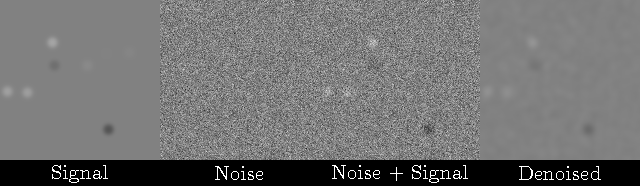
\includegraphics[width=\textwidth]{spectralPhaseRand/primalWeinerDenoise-frame15.png}}\\
\multicolumn{2}{c}{(c) A frame in time of the signal, noise, signal + noise and the Weiner denoised signal}\\
\multicolumn{2}{c}{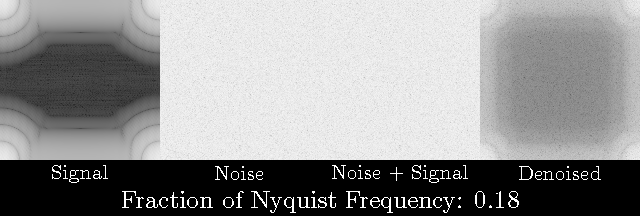
\includegraphics[width=\textwidth]{spectralPhaseRand/freqWeinerDenoise-frame10.png}}\\
\multicolumn{2}{c}{A temporal slice of the 3D FFT the signal, noise, signal + noise and the Weiner denoised signal}\\
\end{tabular}
\caption{The separable spectrum of the signal prior is shown in (a) and (b). The slices can be tensor producted together to reproduce the full 3D spectrum. In (c) and (d), we show the results of Weiner denoising using this spectrum prior. }
\label{fig:weinerMotionNoise}
\end{figure}
